\documentclass[UTF8,a4paper,12pt]{ctexart}

\usepackage{geometry}
\geometry{left=2.35cm,right=2.35cm,top=2.35cm,bottom=2.35cm}
\usepackage{fontspec}
\setmainfont{Tinos}
\setCJKmainfont{Noto Serif CJK SC}
\usepackage{amsmath,amssymb,bm}
\usepackage{siunitx}
\usepackage{booktabs,longtable,array}
\usepackage{graphicx}
\usepackage{float}
\usepackage{subcaption}
\usepackage{xcolor}
\usepackage{listings}
\usepackage[hidelinks]{hyperref}
\usepackage{caption}
\captionsetup{font=small}
\sisetup{detect-all=true,round-mode=places,round-precision=3}

\lstset{
    language=Python,
    basicstyle=\ttfamily\scriptsize,
    keywordstyle=\bfseries,
    commentstyle=\itshape,
    stringstyle=\ttfamily,
    showstringspaces=false,
    breaklines=true,
    frame=single,
    columns=fullflexible,
    tabsize=4
}

\title{太阳电池伏安特性曲线测量实验报告}
\author{Li Jinshuo}
\date{\today}

\begin{document}
\maketitle

\begin{abstract}
本实验测量太阳电池在不同辐照度、不同连接方式下的伏安特性曲线. 实验数据来自七个 CSV 文件, 包括三组单块电池、两组简单串并联电池组以及两组复杂连接电池组. 数据处理用 Python 完成: 读取原始 $U-I$ 数据, 逐点计算 $P=UI$, 由原始测量点确定开路电压、短路电流、最大功率点、填充因子和转换效率, 并采用保形三次 Hermite 插值绘制平滑的 $I-V$ 与 $P-V$ 曲线. 作图时, 单块电池、串联和并联数据统一画在一组图中, 两组复杂连接数据另成一组图. 结果表明, 单块电池的短路电流随辐照度升高显著增大, 开路电压变化较小; 串联主要提高输出电压, 并联主要提高输出电流; 复杂连接的输出功率受弱光电池和支路匹配影响明显.
\end{abstract}

\section{实验目的}

本实验的主要目的如下:
\begin{enumerate}
    \item 测量太阳电池在不同负载电阻下的输出电压 $U$ 和输出电流 $I$, 得到伏安特性曲线.
    \item 根据 $P=UI$ 绘制功率-电压曲线, 找到最大功率点 $(V_m,I_m)$ 和最大输出功率 $P_m$.
    \item 计算开路电压 $V_{oc}$、短路电流 $I_{sc}$、填充因子 $FF$ 和光电转换效率 $\eta$.
    \item 比较不同辐照度对单块太阳电池输出特性的影响.
    \item 比较串联、并联以及复杂连接方式下太阳电池组的输出规律, 并分析其与理想串并联规律之间的差异.
\end{enumerate}

\section{实验原理}

太阳电池可近似看作受光照的 PN 结. 光子入射到半导体材料后产生电子-空穴对, 在结区内建电场的作用下被分离, 从而形成光生电流. 当外部接入负载时, 太阳电池便可以对外输出电功率. 理想单二极管模型可写为
\begin{equation}
    I = I_{ph} - I_0\left[\exp\left(\frac{qV}{n k_B T}\right)-1\right],
    \label{eq:diode}
\end{equation}
其中 $I_{ph}$ 为光生电流, $I_0$ 为反向饱和电流, $q$ 为元电荷, $k_B$ 为玻尔兹曼常数, $T$ 为热力学温度, $n$ 为理想因子. 实际太阳电池还存在串联电阻、并联漏电阻、接触电阻、温度升高和光照不均匀等影响, 因而实验曲线通常只与式 \eqref{eq:diode} 的趋势相符, 而不会完全重合.

太阳电池的工作点由负载决定. 当负载电阻很小时, 电路接近短路, 输出电压接近 $0$, 输出电流接近短路电流 $I_{sc}$. 当负载电阻很大时, 电路接近开路, 输出电流接近 $0$, 输出电压接近开路电压 $V_{oc}$. 在这两个极限之间, 输出功率
\begin{equation}
    P=UI
\end{equation}
先随电压升高而增大, 到达最大功率点后再因电流快速下降而减小. 本实验原始数据中电压单位为 V, 电流单位为 mA, 因此功率可直接写成
\begin{equation}
    P(\mathrm{mW})=U(\mathrm{V})I(\mathrm{mA}).
\end{equation}
最大功率点满足
\begin{equation}
    P_m=V_mI_m=\max\{UI\}.
\end{equation}
填充因子定义为
\begin{equation}
    FF=\frac{P_m}{V_{oc}I_{sc}}.
    \label{eq:ff}
\end{equation}
当 $P_m$ 用 mW 表示、$V_{oc}$ 用 V 表示、$I_{sc}$ 用 mA 表示时, 式 \eqref{eq:ff} 的分子和分母单位均为 mW, 可直接相除. 填充因子越大, 表明 $I-V$ 曲线越接近理想矩形, 电池在最大功率点附近的输出能力越好.

单块太阳电池的长、宽分别为
\begin{equation}
    a=\SI{5.45}{cm},\qquad b=\SI{5.95}{cm},
\end{equation}
因此单块电池面积为
\begin{equation}
    A=ab=5.45\times 5.95\ \mathrm{cm^2}=32.4275\ \mathrm{cm^2}=3.24275\times 10^{-3}\ \mathrm{m^2}.
    \label{eq:area}
\end{equation}
若一个电池组中各电池受到的辐照度分别为 $E_1,E_2,\cdots,E_N$, 则入射光功率取为
\begin{equation}
    P_{in}=A\sum_{j=1}^{N}E_j.
    \label{eq:pin}
\end{equation}
光电转换效率为
\begin{equation}
    \eta=\frac{P_m}{P_{in}}\times 100\%.
    \label{eq:eta}
\end{equation}
代入式 \eqref{eq:eta} 时, $P_m$ 需由 mW 换算为 W.

\section{实验数据与处理方法}

本实验使用七个 CSV 文件作为数据来源. 每个文件包含两列原始测量数据: 第一列为 $U(\mathrm{V})$, 第二列为 $I(\mathrm{mA})$. 表 \ref{tab:data-files} 列出各数据文件对应的实验条件. 原始数据完整列于附录 \ref{sec:raw-data}; 另随报告单独给出可打印的原始数据 PDF 文件.

\begin{table}[H]
\centering
\caption{实验数据文件与对应实验条件}
\label{tab:data-files}
\small
\resizebox{\textwidth}{!}{%
\begin{tabular}{ll}
\toprule
数据文件 & 实验条件 \\
\midrule
\texttt{single-0365W-per-m\textasciicircum{}2.csv} & 单块电池, 辐照度 $\SI{365}{W/m^2}$ \\
\texttt{single-0697W-per-m\textasciicircum{}2.csv} & 单块电池, 辐照度 $\SI{697}{W/m^2}$ \\
\texttt{single-1173W-per-m\textasciicircum{}2.csv} & 单块电池, 辐照度 $\SI{1173}{W/m^2}$ \\
\texttt{serial-749W+653W-per-m\textasciicircum{}2.csv} & 两块电池串联, 辐照度 $\SI{749}{W/m^2}$ 与 $\SI{653}{W/m^2}$ \\
\texttt{parallel-757W+653W-per-m\textasciicircum{}2.csv} & 两块电池并联, 辐照度 $\SI{757}{W/m^2}$ 与 $\SI{653}{W/m^2}$ \\
\texttt{complex1s3p-352W+644W+268W+755W-per-m\textasciicircum{}2.csv} & 一块单电池与三块并联电池串联, 辐照度依次为 $\SI{352}{W/m^2}$, $\SI{644}{W/m^2}$, $\SI{268}{W/m^2}$, $\SI{755}{W/m^2}$ \\
\texttt{complex2p2s-752W+266W+652W+356W-per-m\textasciicircum{}2.csv} & 复杂二串二并等效连接, 辐照度依次为 $\SI{752}{W/m^2}$, $\SI{266}{W/m^2}$, $\SI{652}{W/m^2}$, $\SI{356}{W/m^2}$ \\
\bottomrule
\end{tabular}%
}
\end{table}

数据处理流程如下:
\begin{enumerate}
    \item 用 Python 读取每个 CSV 文件, 将列名统一为 \texttt{U\_V} 与 \texttt{I\_mA}, 并逐点计算 $P=UI$.
    \item 以 $U$ 最接近 $0$ 的测量点作为短路点, 取其电流为 $I_{sc}$; 以 $I$ 最接近 $0$ 的测量点作为开路点, 取其电压为 $V_{oc}$.
    \item 在所有原始测量点中寻找功率最大值, 得到 $V_m,I_m,P_m$. 本报告的参数表全部由原始测量点计算, 不用插值点替代测量点.
    \item 根据式 \eqref{eq:ff} 计算填充因子, 根据式 \eqref{eq:pin} 和式 \eqref{eq:eta} 计算转换效率.
    \item 作图时先按电压升序整理数据, 对重复电压取平均电流, 再用保形三次 Hermite 插值绘制平滑曲线. 插值只用于曲线可视化, 不改变表格中的实验参数.
\end{enumerate}

以 \texttt{single-0697W-per-m\textasciicircum{}2.csv} 为例, 由原始数据得到
\begin{align}
    P_{in} &= EA = 697\times 3.24275\times 10^{-3}\ \mathrm{W}=2.2602\ \mathrm{W}, \\
    P_m &= V_mI_m = 2.33\times 31.55\ \mathrm{mW}=73.5115\ \mathrm{mW}, \\
    FF &= \frac{73.5115}{3.34\times 33.96}=0.648, \\
    \eta &= \frac{73.5115\times 10^{-3}}{2.2602}\times 100\%=3.25\%.
\end{align}
该例说明, 功率曲线的纵坐标可由 V 与 mA 直接相乘得到 mW; 但计算效率时必须将 mW 换算为 W.

\section{实验结果}

\subsection{参数汇总}

\begin{table}[H]
\centering
\caption{由原始 CSV 数据得到的主要光伏参数}
\label{tab:summary}
\small
\resizebox{\textwidth}{!}{%
\begin{tabular}{lrrrrrrr}
\toprule
实验条件 & $V_{oc}$/V & $I_{sc}$/mA & $V_m$/V & $I_m$/mA & $P_m$/mW & $FF$ & $\eta$/\% \\
\midrule
单块, $365\,\mathrm{W/m^2}$ & 3.25 & 18.76 & 2.45 & 17.40 & 42.63 & 0.699 & 3.60 \\
单块, $697\,\mathrm{W/m^2}$ & 3.34 & 33.96 & 2.33 & 31.55 & 73.51 & 0.648 & 3.25 \\
单块, $1173\,\mathrm{W/m^2}$ & 3.35 & 38.15 & 2.41 & 36.28 & 87.43 & 0.684 & 2.30 \\
两块串联, $749+653\,\mathrm{W/m^2}$ & 6.56 & 20.20 & 5.75 & 17.98 & 103.39 & 0.780 & 2.27 \\
两块并联, $757+653\,\mathrm{W/m^2}$ & 3.28 & 39.27 & 2.79 & 36.80 & 102.67 & 0.797 & 2.25 \\
$1S+3P$, $352+644+268+755\,\mathrm{W/m^2}$ & 6.45 & 18.30 & 5.86 & 16.43 & 96.28 & 0.816 & 1.47 \\
$2S2P$, $752+266+652+356\,\mathrm{W/m^2}$ & 6.46 & 36.31 & 5.56 & 33.45 & 185.98 & 0.793 & 2.83 \\
\bottomrule
\end{tabular}%
}
\end{table}

从表 \ref{tab:summary} 可见, 单块太阳电池的 $I_{sc}$ 随辐照度由 $\SI{365}{W/m^2}$ 增至 $\SI{1173}{W/m^2}$ 而由 $\SI{18.76}{mA}$ 增至 $\SI{38.15}{mA}$, 增幅明显. 相比之下, $V_{oc}$ 仅由 $\SI{3.25}{V}$ 增至 $\SI{3.35}{V}$, 变化很小. 这与太阳电池理论一致: 光生电流近似随光照增强而增大, 而开路电压对光生电流呈对数依赖, 因而变化较缓慢.

两块电池串联时, $V_{oc}=\SI{6.56}{V}$, 约为单块电池开路电压的两倍, 而 $I_{sc}=\SI{20.20}{mA}$ 与单块电池电流量级相近. 两块电池并联时, $V_{oc}=\SI{3.28}{V}$, 与单块电池相近, 但 $I_{sc}=\SI{39.27}{mA}$ 明显增大. 因此, 串联主要提高输出电压, 并联主要提高输出电流.

\subsection{$I-V$ 曲线}

\begin{figure}[H]
\centering
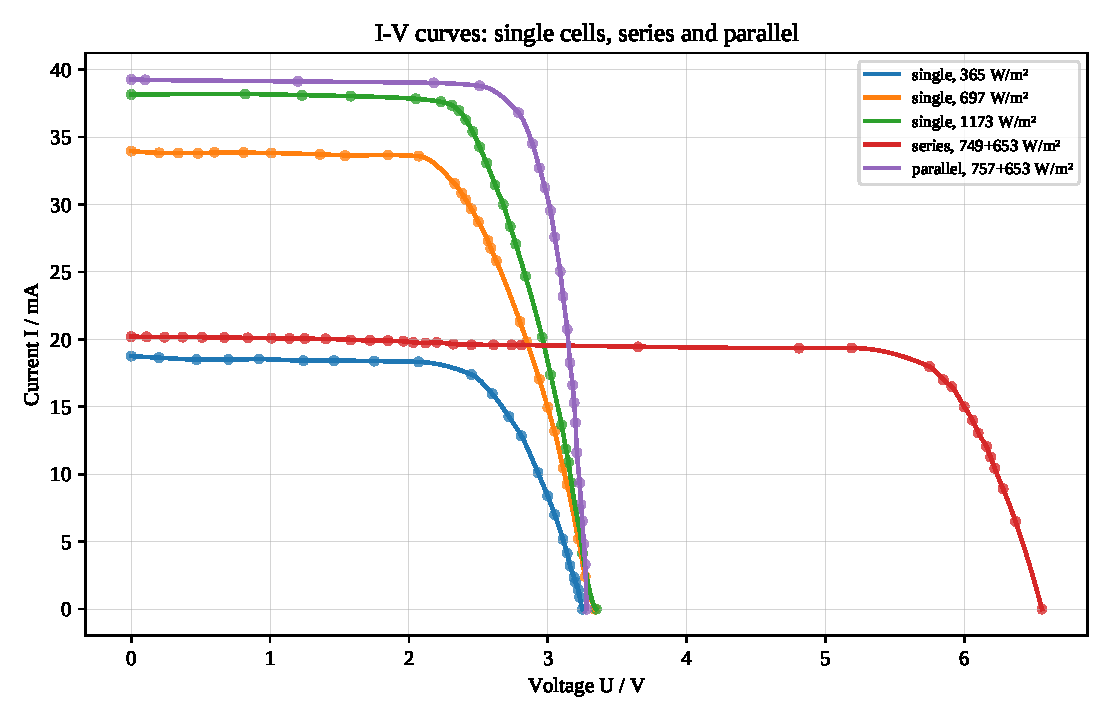
\includegraphics[width=0.92\textwidth]{figures/non_complex_iv.pdf}
\caption{单块电池、两块串联和两块并联数据合并绘制的 $I-V$ 曲线}
\label{fig:non-complex-iv}
\end{figure}

图 \ref{fig:non-complex-iv} 将三组单块电池和两组简单连接电池组画在同一张图中. 单块电池随辐照度升高表现为曲线整体上移, 即相同电压下输出电流增大. 两块串联曲线的电压范围扩展到约 $\SI{6.56}{V}$, 但低压区电流仍保持在约 $\SI{20}{mA}$; 两块并联曲线的电压范围仍接近单块电池, 但低压区电流提高到约 $\SI{39}{mA}$. 这说明串联与并联改变的是输出电压和输出电流的分配方式.

\begin{figure}[H]
\centering
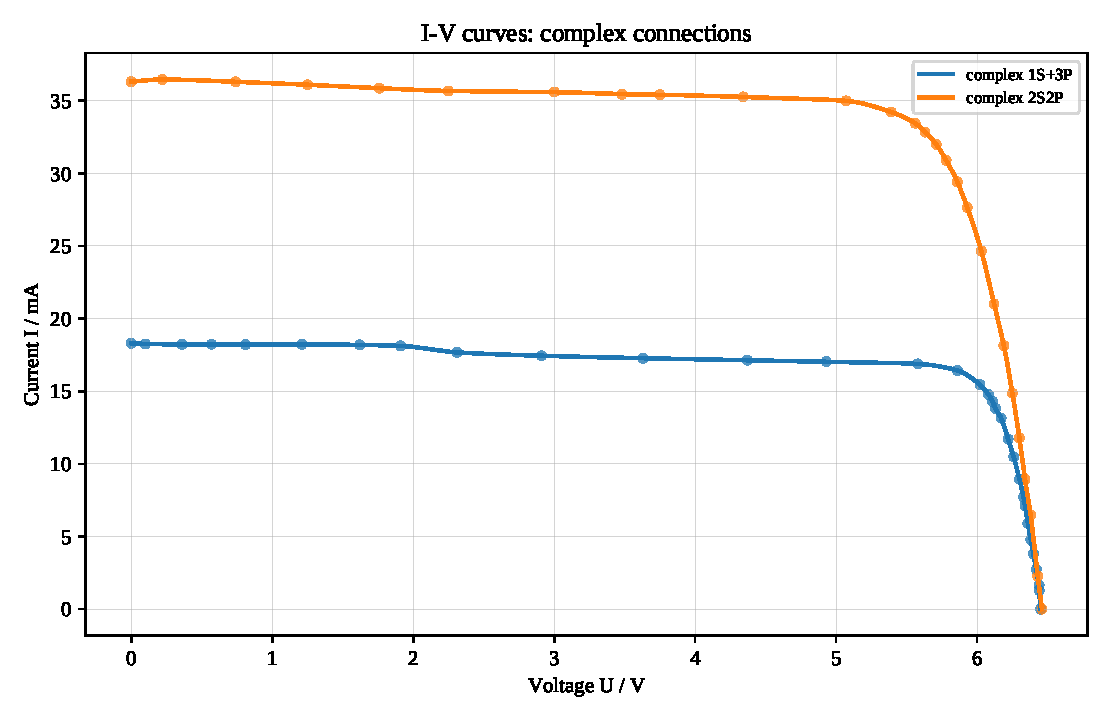
\includegraphics[width=0.92\textwidth]{figures/complex_iv.pdf}
\caption{两组复杂连接数据单独绘制的 $I-V$ 曲线}
\label{fig:complex-iv}
\end{figure}

图 \ref{fig:complex-iv} 比较两种复杂连接方式. 二者开路电压都约为 $\SI{6.45}{V}$, 说明等效结构都包含串联增压特征. 但 $2S2P$ 的短路电流约为 $\SI{36.31}{mA}$, 显著高于 $1S+3P$ 的 $\SI{18.30}{mA}$. 这表明 $1S+3P$ 中串联单电池对总电流有明显限制, 而 $2S2P$ 具有更强的电流输出能力.

\subsection{$P-V$ 曲线}

\begin{figure}[H]
\centering
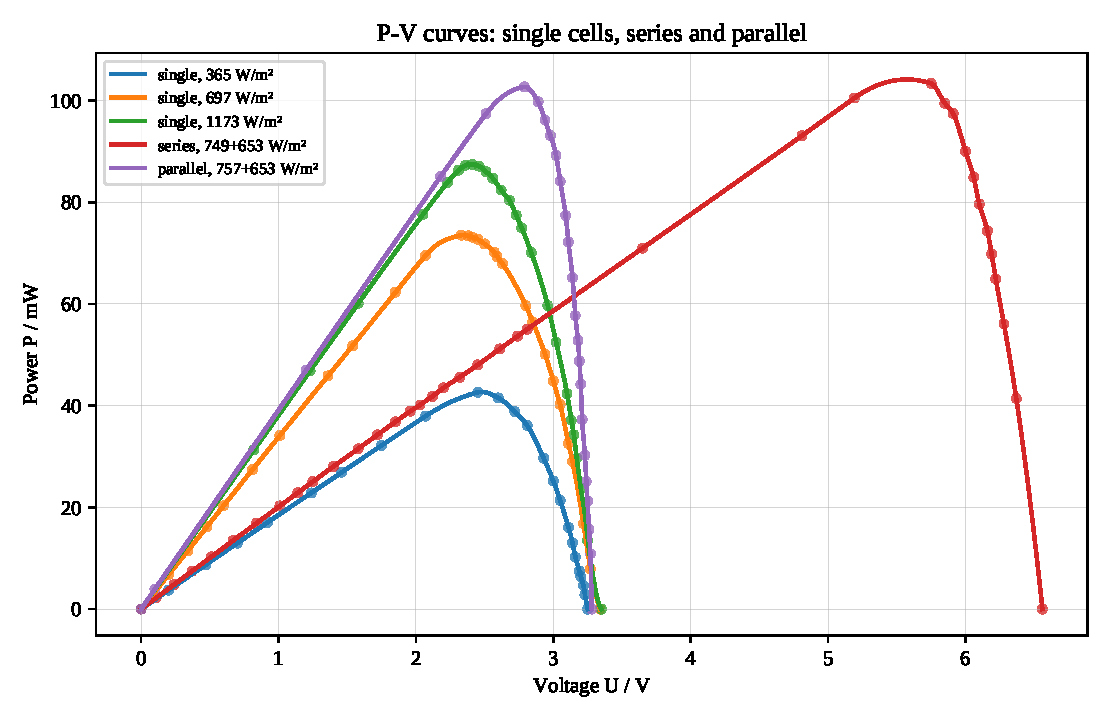
\includegraphics[width=0.92\textwidth]{figures/non_complex_pv.pdf}
\caption{单块电池、两块串联和两块并联数据合并绘制的 $P-V$ 曲线}
\label{fig:non-complex-pv}
\end{figure}

图 \ref{fig:non-complex-pv} 中, 各曲线均表现为功率先上升后下降. 这是因为低电压区虽然电流较大, 但电压过低; 高电压区虽然电压较大, 但电流迅速下降; 因此最大功率点位于曲线拐弯区域附近. 两块串联与两块并联的最大输出功率分别为 $\SI{103.39}{mW}$ 和 $\SI{102.67}{mW}$, 数值非常接近. 这说明在入射总光功率相近时, 串联和并联不必然显著改变最大可输出功率, 而主要改变输出的电压-电流组合形式.

\begin{figure}[H]
\centering
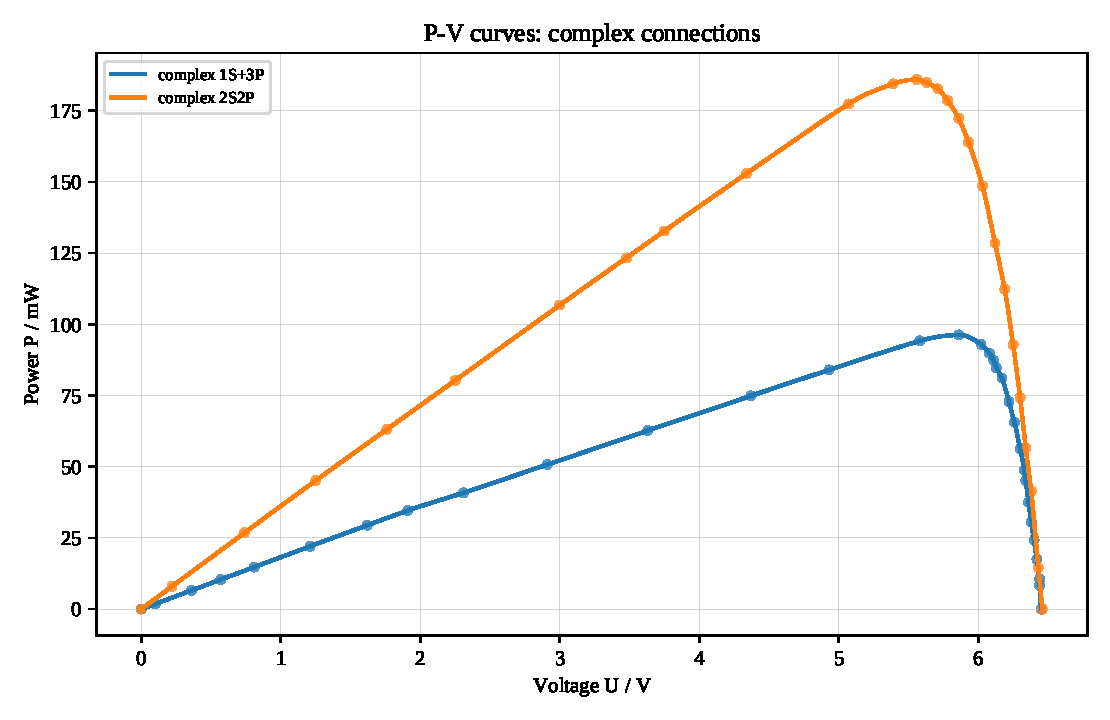
\includegraphics[width=0.92\textwidth]{figures/complex_pv.pdf}
\caption{两组复杂连接数据单独绘制的 $P-V$ 曲线}
\label{fig:complex-pv}
\end{figure}

图 \ref{fig:complex-pv} 显示, $2S2P$ 的最大功率为 $\SI{185.98}{mW}$, 明显高于 $1S+3P$ 的 $\SI{96.28}{mW}$. 尽管两组实验的入射总辐照度相近, 但 $1S+3P$ 中单块串联电池会限制整个串联支路的电流, 且三并联部分中存在弱光电池, 导致整体输出受限. $2S2P$ 则兼具较高电压和较高电流, 因而输出功率更大.

\section{误差分析与结果讨论}

\subsection{辐照度和温度的影响}

理论上, 短路电流与辐照度近似成正比, 开路电压随辐照度呈对数增长. 本实验中 $I_{sc}$ 从 $\SI{18.76}{mA}$ 增至 $\SI{38.15}{mA}$, 体现出明显的光照增强效应. 但从 $\SI{697}{W/m^2}$ 到 $\SI{1173}{W/m^2}$, $I_{sc}$ 只由 $\SI{33.96}{mA}$ 增至 $\SI{38.15}{mA}$, 低于简单线性预期. 可能原因包括: 强光下电池温度升高导致载流子复合增强; 光源不是标准太阳光谱; 电池表面光照分布不均匀; 大电流下内阻和接触电阻造成的压降更加明显.

\subsection{串并联不匹配}

串联电池组的总电流容易被最弱电池限制. 如果两块电池辐照度不同, 弱光电池会限制整个串联支路的电流, 在复杂阵列中还可能形成局部反向偏置. 并联电池组的端电压基本相同, 但各支路的电流分配取决于电池自身参数、光照强度和内阻. 因此, 复杂连接的输出不能简单地把单块电池参数线性相加, 而应考虑支路匹配、光照均匀性和内阻损耗.

\subsection{测量和作图误差}

本实验主要误差来源包括:
\begin{enumerate}
    \item 电阻调节和读数过程存在时间延迟, 太阳电池温度可能在测量过程中不断变化.
    \item 电压表、电流表和导线接触电阻会影响实际负载工作点.
    \item 部分曲线拐点附近数据点仍不够密集, 最大功率点可能略偏离真实连续曲线最大值.
    \item 作图使用插值平滑曲线, 其目的只是改善可视化效果. 插值曲线不代表精确物理模型, 因此最大功率点仍应以原始测量点为准.
\end{enumerate}

\section{反思总结}

本实验说明, 太阳电池的输出能力不仅取决于辐照度, 也取决于连接方式和电池之间的一致性. 对单块电池而言, 增强光照主要提高短路电流, 对开路电压的影响较弱. 对多个电池而言, 串联适合提高输出电压, 并联适合提高输出电流. 但在复杂连接和不均匀光照条件下, 弱光电池和不匹配支路会限制整体输出, 使实际最大功率明显低于简单叠加预期.

从数据处理角度看, 本实验不应只画 $I-V$ 曲线, 还必须画 $P-V$ 曲线. 因为最大功率点在 $I-V$ 图中不一定直观, 而在 $P-V$ 图中可以直接读取. 此外, 参数计算应尽量基于原始数据点, 避免把平滑插值产生的点误当作真实测量值.

\section{延伸探讨}

若要进一步提高实验精度, 可以从以下方面改进:
\begin{enumerate}
    \item 在电池背面加温度传感器, 同时记录温度, 研究 $V_{oc}$ 和最大功率点随温度变化的规律.
    \item 在最大功率点附近增加负载取点密度, 或使用电子负载连续扫描, 以更准确地确定 $P_m$.
    \item 分别测量每一块电池的单独 $I-V$ 曲线, 再与串并联后的整体曲线对比, 从而定量分析不匹配损失.
    \item 对复杂连接阵列建立等效电路模型, 将每块电池表示为光生电流源、二极管和内阻的组合, 再通过数值方法求解阵列输出曲线.
\end{enumerate}

\appendix
\section{原始数据}
\label{sec:raw-data}

以下各表列出所有 CSV 文件中的原始 $U-I$ 数据. 其中 $P=UI$ 为根据原始电压和电流逐点计算得到的功率, 用于功率曲线绘制和最大功率点查找.

\input{raw_data_tables.tex}

\end{document}
